\Chapter{Problems}{Claire Court}

At this point it seems to be the moment to give a brief account for the sake of anyone who might be interested, of what it is like actually running a shop. There must be many other people without previous trading experience who have taken over village Post Offices and stores, though perhaps not built over the ashes of their ancestors. They no doubt would be able to add much to what I am about to disclose - not that there is anything particularly sensational to reveal, merely a sizeable collection of small things, some pleasant and some less so. It will probably seem laughable to many readers but at the beginning of our new venture we actually bought a "Teach Yourself" book of shopkeeping - it probably contained good advice but all the conclusions I have since formed have been based on practical and not academic knowledge. Most of the information of which I am about to disburden myself was gleaned between 1968 and 1971. At the time it seemed much longer than three years.

There is no denying that one of the most satisfying and important aspects of shopkeeping is the feeling that all the hard work and effort one puts into it is for oneself and one's own family, rather than for an employer or an impersonal organisation. It is this independence which sustains many small shopkeepers who exist on tiny profits in the face of rising overheads and cut-throat competition. Another advantage which is not to be despised is the convenience of being able to buy goods at cost price. The profit on footwear is reckoned to be thirty per cent out of which taxes and overheads, such as postage, have to be paid. When we first began trading, thirty per cent seemed to us to be a very good profit but it was not long before we discovered the snags - the many pairs of shoes for example which never find a buyer and are left on the shelves; coloured slippers which quickly lose their newness and fade when displayed in the window; the occasional faulty pair of shoes which has to be returned to the wholesaler by post usually unless one is lucky enough to catch the traveller and obtain credit. We very soon came to learn that the nominal thirty per cent in reality represents a very much smaller profit than it would seem at first sight; quite apart from the wear and tear on one’s own constitution. We never claimed anything out of the business as payment for the many hours of work that we put in to it, and after enduring a year or two of back breaking labour for very small financial returns, we began to feel increasingly reluctant to continue such a thankless task.

One must not forget, though, the satisfaction of completing the task of rearrangement, of making a pleasing display of all the brightly coloured slippers, toys and fancy goods in the window. Even in a small village like ours it was surprising how much interest was shown in our activity every time it became apparent that we were taking all the goods out of the window and altering the arrangement, it was impossible to work late at night without the whole of Lower Washford knowing about it as the light from the large window shone forth like a beacon, and we could be sure that at least one customer next day would make a special little journey up the road by Walnut Tree to see what we had been doing.

I have mentioned how we enjoyed visiting wholesalers and trade fairs, but this of course was a modern innovation made possible by the motor car and unknown to parents or grandparents. Trade had always been conducted in a very leisurely and courteous fashion with travellers, whose visits came around about three or four times a year. In theory at least if not in practice one is expecting the traveller when he calls, for he usually announces his intended visit by post card a few days before his appearance and there is an unwritten rule that he will collect any outstanding payments with his fresh order. Over the years of trading many travellers had become like old friends to William and Ada and Aunt Selina, and their visits were welcome until the last few difficult years, when both parties knew that to make an old lady add more stock to what was already mouldering away in corners of the shop was about the last thing any sympathetic person would wish to do. Some of the travellers of course were more likeable than others, and we were suitably grateful for the one or two who really tried hard to help us find the right stock for our particular shop and did not exploit our innocence.

Journeying from shop to shop in isolated rural areas must be quite a difficult way of making a living as often our modest stationery order would not come to more than five or six pounds gross, and even this would have taken perhaps over an hour of the traveller's time. Yes - although I frequently groaned inwardly at the arrival of the traveller, who through no fault of his own tended to drop in at the wrong moment, now that they no longer call, I miss them!

I have already spoken of the close personal relationship which had always existed between shopkeeper and customer. Postmistresses of course are notorious for knowing everyone's business but it must be said for Ada that she very rarely discussed the private business of her customers with us. A very different relationship existed between ourselves and the later generation of villagers. I was not local which put me at a disadvantage straight away and the twin barriers of education and a twenty year absence from the village were well-nigh impossible to bridge. We struggled manfully, but both sides knew that we did not speak the same language. Not only did we not know the villagers names, who had married whom and how many children they had, but we found it difficult to summon up much interest in such matters.

One of the disadvantages of shopkeeping too, which we had hopelessly underestimated, was the amount of effort which is required to keep the shop itself clean and reasonably tidy. The glass counter had to be polished, the window had to be turned out from time to time and rearranged, and shoes which had been tried on had to be put back in their correct boxes and replaced on the shelves. All this takes time and energy, but it was completely uneconomic to employ anyone to perform these simple tasks for me. So on many and many a weary evening we laboured away, making price tickets, propping up toys or gifts which wanted to fall down, and wrestling with tiresome little peg board fittings. 

Cleaning the window of the shop was an operation which was fraught with not inconsiderable hazard, the first of which was its size and height, and second, its close proximity to the road. It had been purpose built in order that William should be able to hang up the bicycles he had for sale for generous display space would not have disgraced a town store. There was a stone ledge running around the outside near the base of the window and by dint of clinging on to the supporting struts it was just possible (for I am fairly tall) to reach the top of the window and clean it. After a while I became fairly adept at jumping up and down off the ledge though I never looked forward to doing so as the villagers used to pass facetious remarks when they saw me working. As cleaning the window was rather a dirty job I did not wear my best clothes for it, and usually protected my hair with a cotton sunhat. Imagine my annoyance one day when just jumping down from my perch, girded with my armoury of dusters and brushes, not forgetting the hat, my eyes met those of a senior school colleague just driving past in his car! I had always kept my two lives completely separate, but truth will out sonner or later, and it took a long time for my wounded pride to recover.

And dusting, too, endlessly dusting. Whose idea was it, I used to ask myself, to buy all those Chinese fans and cute little rabbits? How do you get dead flies out of the front of the window, a spot they seem to particularly favour, without knocking over all the jigsaw puzzles, babies shoes and West Country guides that are so carefully arranged between you and them?

Greetings cards are a very steady seller, but why do short sighted senior citizens come in to buy one without their glasses, so that you have to drop everything to read out the verses to them - and then after lengthy consideration, the verses fail to appeal and you do not succeed in selling it. A laborious way indeed of not earning the penny profit. Greetings cards are a real eye-opener where character study is concerned. By the type of card chosen one could (someone probably has) write a small paper on that person's background, education, tastes and social class. Flowers, particularly pink or red roses, are easy winners where cards are concerned. Closely following them in descending order are pictures of puppies, kittens, children, bluebell woods and horses. Humorous cards do not go down well in villages, neither do cards in what we have come to label "good taste", plain colours and lacking an invocation to Grandmother, Granny, Grandma, Gran, Nanny or Nan. Yes, believe it or not, all six appellations are catered for and a card which is not labelled with the relationship of the loved one has little hope of selling. Another pitfall with greetings cards is the rate at which they become soiled and unsaleable, or lose their envelopes, which is one of the reasons for the high price the customers are so ready to complain about.

After we had been keeping the shop for a while, some of the customers started to ask for gardening items such as potting compost and slug pellets. William had always held the agency for Webbs seeds, a very respectable steady seller, though not very profitable in a small business such as ours. One season, out of interest, we worked out our profit on the sale of seeds and after deducting postage for returning the end of season surplus, the sum came to the grand total of 6s. 5d! Gardening is a very popular pastime in villages and there is constant demand for fertiliser, weedkiller and so forth. We found a very good wholesaler in Taunton and were able to get excellent quality goods delivered regularly to order, which was one advantage of living on the main road. This is a part of the business which we thoroughly enjoyed and had we continued trading for a longer period, would probably have worked up quite a good turnover. We kept a few tools as well as flower bulbs and potted begonias and hyacinths at Christmas time. They helped to give the shop a pleasant atmosphere and introduced a new and distinctive earthy aroma, which blended with the old-fashioned homely smell of leather and post office ink.

All the time that this was going on we were endeavouring with partial success to continue our normal lives, I at my teaching post and Glyn at his very demanding job, which entailed working on Saturday mornings. The Saturday business was a very sore point as it was the one day of the week when a few customers used to come in, and this meant that I was completely tied to the shop. Glyn would return home in time for a late lunch at nearly two o-clock and I (by then thoroughly out of humour after a boring morning indoors) used to leave him in charge and go to do my shopping. In reality I was prompted by a desire to get away from everything connected with the shop. Saturday had always been a happy family day on which we would go to town, have a little outing or do our gardening and I do not think I ever forgave the shop for ruining our weekend.

Perhaps it is just as well that life is a mixed affair and even when things were not going well there could be an occasional pleasant and enjoyable day. Take an example, - one might start the morning by selling a pair of shoes, then perhaps a workman would come in for a pair of boots and by a happy chance the size and sort that he wanted was reposing on our shelves. Five pounds in the till - a small miracle! Then perhaps a customer would come in who remembered Glyn as a small boy and there could be much pleasant swapping of reminiscences. The summer season was particularly enjoyable in this way, as long lost friends would occasionally appear with their children, who would oblingingly spend all their pocket money with us. Often, visitors from large towns would be amazed at the low prices of the goods in our shop which cheered us up no end, as the impression given by some of the local customers was that we were fleecing the coats from off their backs and living in luxury on the proceeds.

Every now and again though we would go through a period of hopeless disillusionment over the whole project, and at these times the very sight of the shop would induce a feeling of revulsion. All we wanted to do was to get as far away from it as possible, live a normal life again and have a much needed holiday. After two years, we gave up the Post Office so that we could at least close the shop if we wanted to. Trade dropped off so we took to being closed most of the day and opening at tea-time when the men were on their way home from work. He obviously lost some trade, but quite often, after getting rid of the Post Office, I would stay in the whole morning and not one single customer would appear. There was a bell on the door, but we often did not hear it, as the house is large and the walls are thick. However, most people knew if we were in, and would come to the back door if they wanted something. This dragged on for a while with an occasional burst of success, but after a year or so it became obvious that we would never get rid of all the shoes that we had bought. However, patience is a great virtue where retail trade is concerned. A very good example of this axiom is the story of the cheap ladies calf length boots which Glyn brought back from Bristol one day, early in our ownership before the novelty of trading had worn off. He bought three pairs of those boots and as they were only priced at 39/11 we succeeded in selling two of them fairly easily. The third pair, however, obstinately would not sell which was hardly surprising as they were of a vivid shade of magenta, and had such narrow cut legs, that even would-be purchasers found it quite impossible to get them on. After standing around for a year, these boots became a sort of evil genius, leering at us reproachfully every time we went into the shop. They fell over several times, and on more than one occasion were liberally splashed with floor-washing water. Refusing to stand up on their own they had to be continually propped with rolled newspapers. We tried them by the door, we tried them in the window, we tried them on the counter - nothing worked.

After three years, the village was as bored with them as we were. Eventually, when we were on the last lap of our discount sales and, resigned to living with the boots for ever, I wiped them yet again with a damp cloth, knocked out the dead spiders and remnants of cigarette ash which had found their way inside, and out them in the window with a card declaring that for £1 they were a bargain and - cri de coeur in hope of salvation - suggesting that they should be dyed black. The rest is easy to guess. I was in the garden one Saturday when one of the girls rushed out to me, breathless with excitement, "Mummy, there's a girl in the shop and she's TRYING ON THE PURPLE BOOTS." The atmosphere was heavy with expectation as I rushed back to the scene of action in my gardening clothes. My eyes were drawn, nay riveted, to the important area in the field of action - the girl's legs. Instantly I knew - here at last was the girl I had been waiting for. Thin as a lath, with legs like sticks, she was on her way to the chilly, rainswept seaside, intending to paddle but had forgotten her wellies. Not only were the boots what she needed - she had. obviously fallen in love with them, whereupon Mum oblingingly produced the £1, to the satisfaction of all concerned.

For an hour or two after this the house echoed with the refrain, "We've sold the purple boots!"

Several little morals could be drawn from this story, one of which is that if you wait long enough and patiently enough, eventually you will find a customer for the most unlikely goods. I could tell similar tales of other goods which seemed impossible to sell - round toed men's shoes size 5 1/2 spring to mind, or old fashioned ladies shoes size 2. On a day when your mind is miles away a little old lady or gentleman will come in and be delighted to find the tiny size they require. Perhaps I romanticise but it is almost as if the goods had been waiting patiently all those years to be claimed by their rightful owner, so happy is the moment of discovery when it eventually comes.

At sale time we had continual struggles with oar conscience when it came to trying to price the stock. Often when we took some of the leather boots and shoes from their boxes, not only were they in perfect condition, but prices marked on them seemed so ridiculously low that we felt tempted to alter them just a little. I particularly recall one pair of John White’s gentleman’s light leather boots in a box marked 49/11. They had been on the shelves a few years but as they were perfect we felt that they were worth several pounds in modern money. So just on this pair I (rather naughtily) fixed a label - 69/11 49/11. Not really dishonest, just encouraging the customers a little! All the other shoes I marked at the correct prices. A day or two later, the shop door opened and in came a pleasant, politely spoken man,

\begin{quote}
\textbf{P.P.S.M.}: Good morning, Madam. Are you the owner of the shop? \\
\textbf{Me} (not sure whether greater prudence lay in agreeing or disagreeing):  Well, my husband is, really. \\
\textbf{P.P.S.M.}: Oh well, you’ll do. (No escape!) I just happened to be passing and noticed you had your "Sale" Notices up. \\
\textbf{Me} (in true peasant fashion, not eager to commit myself): Oh - yes, \\
\textbf{P.P.S.M.}:  I'm the Weights and Measures Officer so it seemed a good moment to just stop and have a little chat about the regulations governing reductions and so forth. I find owners of small businesses often don’t realise that they can be breaking the law. 
\end{quote}

He proceeded to explain that it was not permitted to claim genuine reductions on goods unless they had been marked at the higher price for (I think) three months and looking around the shop for an example, in order to show me in the nicest possible way, the pitfalls that await a decent honest trader like myself.

\begin{quote}
\textbf{P.P.S.M.}:  You see, Madam, say you had altered the price on a pair of shoes say from £3 to £4- and then crossed it out, that would be against the law. \\
\textbf{Me}  (feeling rather uncomfortable): Yes, I see your point - but what about the rise in the cost of everything? Some of these boots and shoes are worth a lot more than they’re marked and we have to pay rates etc. Aren’t we allowed to put the price up at all? \\
\textbf{P.P.S.M.}: Oh yes, indeed, but you must prove that they had been marked up a month before you held your sale. (Looking round once more for an example) Now, take that pair of boots (upon which he fastened on the very pair I have mentioned, the one guilty felon in all that innocent looking row). Say you had just marked that up and then crossed out the price - that would be illegal.
\end{quote}

How I did not blush I shall never know, I was quite expecting him to demand to see the empty box the boots had occupied on which was plainly marked the cipher 49/11, but after continuing to tighten the screws a few seconds longer, he let me off the rack and proceeded to other matters.

For weeks afterwards I awaited his reappearance with bated breath but he never came back. I think he was genuinely unaware of my discomfiture but I never quite made out how he came to pick on that one pair of rather old-fashioned but worthy boots of all the dozens of pairs on display. I think my mind must have been concentrating on them to such an extent that his hand was guided in their direction. A narrow escape indeed - but it had the effect of making us much more careful afterwards.

This dragged on for a while and then at this point fate stepped in and on the 9th May 1971 the unbelievable happened. On one of the ill-starred Saturdays, fire broke out in the back room of the shop. While the children and I were shopping in Minehead, we learnt of the fire from neighbours. Rushing home we found that the blaze was already extinguished. In the midst of the charred and evil-smelling mess our feelings were unanimous - shock, horror and incredulity, but more than anything, an overpowering sense of relief. We had tried hard but this was the unforeseen end of a long and painful chapter.

\begin{figure}
	 \centering
     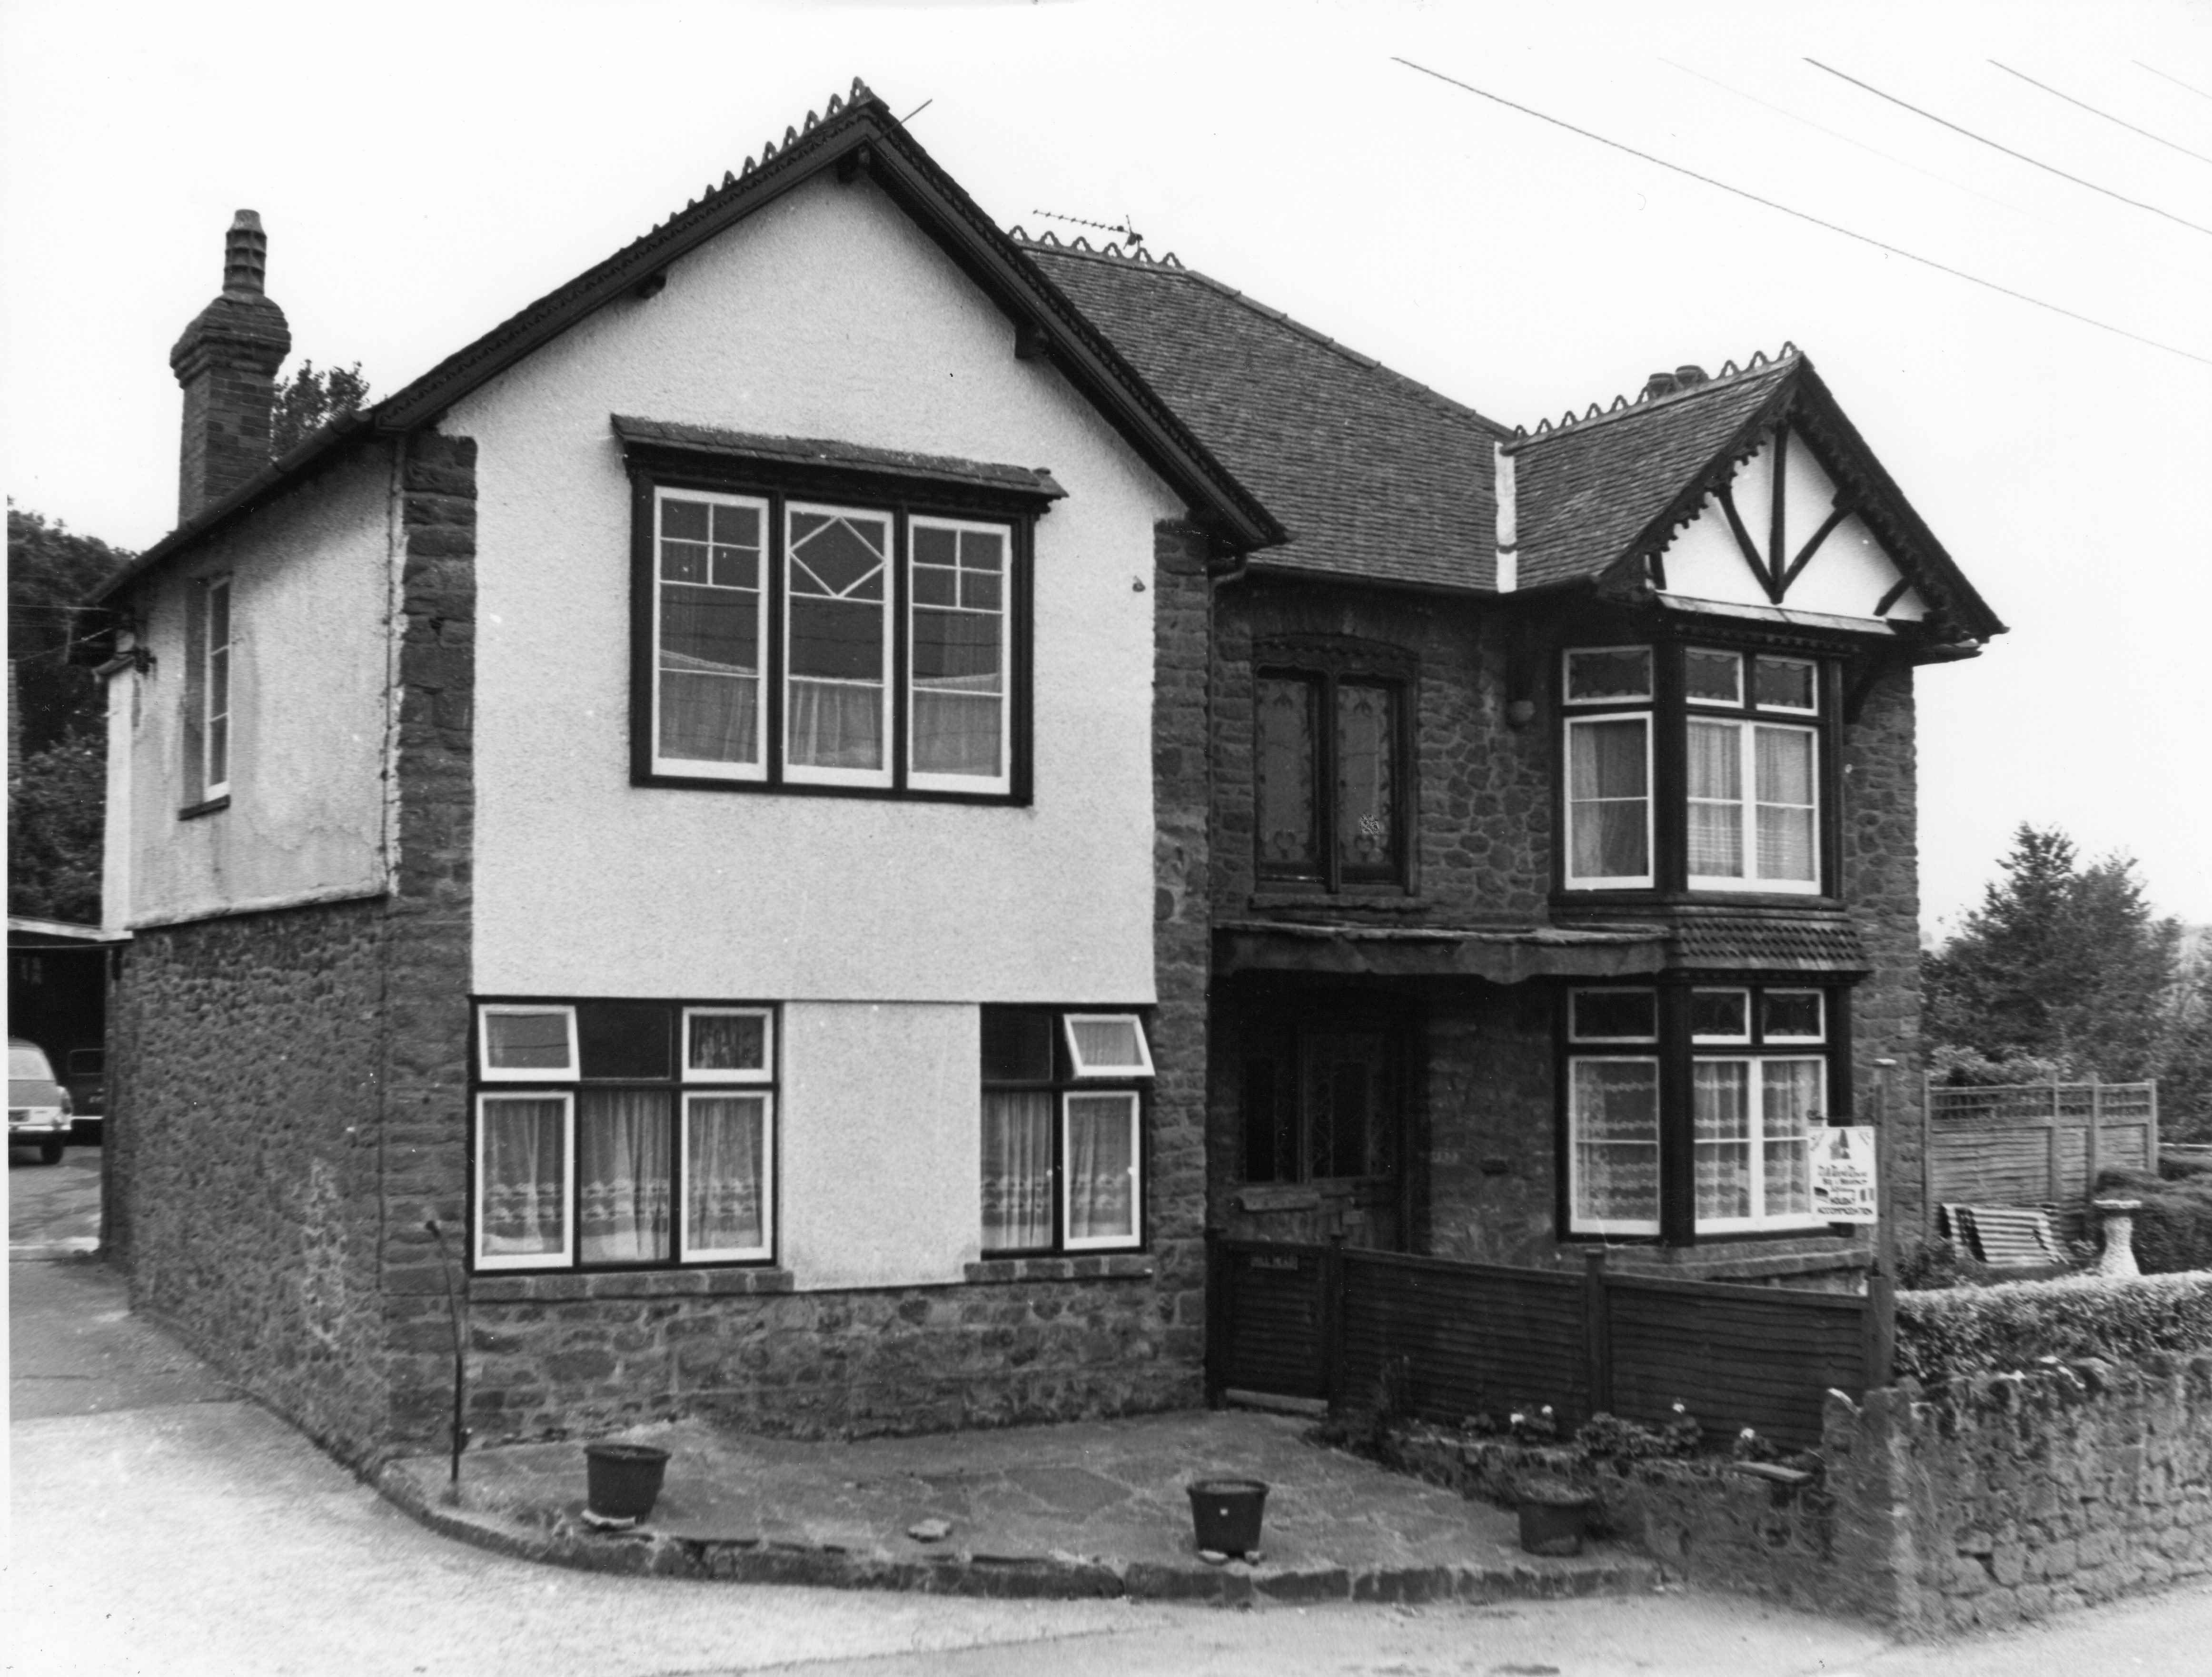
\includegraphics[width=1\textwidth]{figures/HillHeadHouse1970}
     \caption{The house, shortly after restoration from the fire and conversion of the shop}
     \label{fig:House1970}
\end{figure}

